\documentclass[9pt,pdf,hyperref={unicode}]{beamer}
\beamertemplatenavigationsymbolsempty

\setbeamertemplate{blocks}[rounded=true, shadow=true]
\setbeamertemplate{footline}[page number]
\usepackage{multicol}

\usefonttheme{serif}

\usepackage[utf8]{inputenc}
\usepackage[english, russian]{babel}
\usepackage{amsmath,mathrsfs,mathtext}
\usepackage{graphicx, epsfig}
\usepackage{caption}
\usepackage{subfig}
\usepackage{amsmath, bm}

\usepackage{comment}

\usepackage{tabularx}

\usepackage{tikz}

\DeclareMathOperator*{\argmin}{arg\,min}
\DeclareMathOperator*{\argmax}{arg\,max}

\makeatletter
\let\@@magyar@captionfix\relax
\makeatother

\usetheme{Warsaw}
\usecolortheme{sidebartab}
\definecolor{beamer@blendedblue}{RGB}{31,96,49}

\setbeamertemplate{enumerate items}[circle]

\setbeamersize{text margin left=1.5em, text margin right=1.5em}

\usepackage{ragged2e}
\usepackage{algorithm}
\usepackage{algpseudocode}

%----------------------------------------------------------------------------------------------------------
\title[\hbox to 56mm{Decentralized Domain Adaptation \hfill\insertframenumber\,/\,\inserttotalframenumber}]
{Decentralized Domain Adaptation}
\author[Шокоров В.\ А.]{\Large Шокоров Вячеслав Александрович}
\institute{ Московский физико-технический институт\\
Факультет управления и прикладной математики\\
Кафедра интеллектуальных систем\\
~\\
Научный руководитель д.ф.-м.н. В.\,В.~Стрижов
}

\date{\footnotesize{\emph{Москва}\\
 2020 г}}
%----------------------------------------------------------------------------------------------------------
\begin{document}
%----------------------------------------------------------------------------------------------------------
\begin{frame}
\titlepage
\end{frame}

%--------------------------------------------------------------------------------------------------------
\begin{frame}{Цель исследования}

\begin{block}{Цель} 
Построить теоретического обоснования приминения подхода transfer learning для задачи доменной адаптации. \end{block}

~\\
\begin{block}{Проблема}
Латентные вероятностные пространства очень запутаны, например пространства моделей GAN часто имеют семантически значимые направления. Из этого следует, что модели могут раскладывать все вероятностное пространство на наиболее значимые компоненты. И мы хотим понять, насколько релевантно использование предобученных моделей которые уже умеют находить эти компоненты.
\end{block}

\end{frame}

%--------------------------------------------------------------------------------------------------------
\begin{frame}{Цель исследования}

\begin{block}{Решение}
Докажем следующие теоремы: 
    \begin{itemize}
        \item[$\mathbf{Th_1}$] (О стабилизация результата):
        Существует модель, которая строит достаточно качественное инвариантное представление вероятностного пространства, что для нее существует сходимость по итерациям обучения к логарифму правдоподобия, независящего от домена.
        \item[$\mathbf{Th_2}$] (О неуменьшение точности): 
        Для модели из первой теоремы, верно, что при ее увеличении ее сложности наблюдается неуменьшение точности предсказания. 
        \item[$\mathbf{Th_3}$] (О возможном уменьшения обучающей выборки): 
        Для модели,  из первой теоремы, верно, что при смене домена для стабилизации математического ожидания и дисперсии достаточен меньший объем выборки.
    \end{itemize}
\end{block}

\end{frame}

%--------------------------------------------------------------------------------------------------------
\begin{frame}{Теоретическая часть}
	    Задача доменной адаптации это задача одноклассовой классификации. \\
        Есть веротностное пространство $\mathcal{X}$, которое полученое компизицией двух функций $f$ и $g$, где $f$ задает класс объетка, а $g$ пораждает шум (домен). Например $f$~--- задает класс -  самолет, функция $g_1$ переводит класс самолет в картинку модели, а функция $g_2$ переводит в изображение настоящего самолета. \\
        Мы хотим научиться обучать модель так, чтобы мы могли определять класс объекта при изменении функции $g$, возможно с небольшим дообучением. 

    \begin{figure}[h]
        \begin{minipage}[h]{0.89\linewidth}
        \center{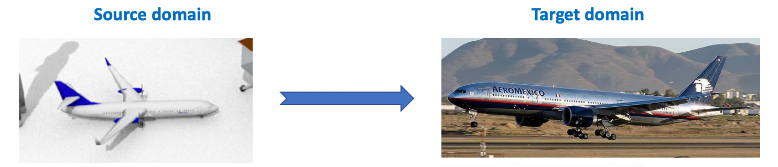
\includegraphics[width=1\textwidth]{pictures/source-target_domen.png}}
        \end{minipage}
    \label{heat_maps}
    \end{figure}

    Задача может быть сформулирована в терминах Few-Shot или Zero-Shot Learning.      
\end{frame}
%----------------------------------------------------------------------------------------------------------
	\begin{frame}{Список литературы}
		\begin{thebibliography}{1}
			
			\bibitem{GraphSAGE}
			\BibAuthor{Ben-David, S., Blitzer, J., Crammer, K. et al. A theory of learning from different domains. Mach Learn 79, 151-175 (2010). https://doi.org/10.1007/s10994-009-5152-4}

			\bibitem{wilson2020survey}
			\BibAuthor{Garrett Wilson and Diane J. Cook}
			\BibTitle{A Survey of Unsupervised Deep Domain Adaptation}
			\BibVolume{arXiv/1812.02849} 2020
			
			\bibitem{kouw2019introduction}
			\BibAuthor{Wouter M. Kouw and Marco Loog}
			\BibTitle{An introduction to domain adaptation and transfer learning}
			\BibVolume{arXiv/1812.11806} 2019
			
		\end{thebibliography}
		
	\end{frame}

%----------------------------------------------------------------------------------------------------------
\begin{frame}{Пример релевантности задачи}
    На картинке показано, что изменения вдоль определенных, выделенных направлений в латентном пространстве GAN-а дает смену домена, что показывает корректность задачи. 
    
    \begin{figure}[h]
        \begin{minipage}[h]{0.59\linewidth}
        \center{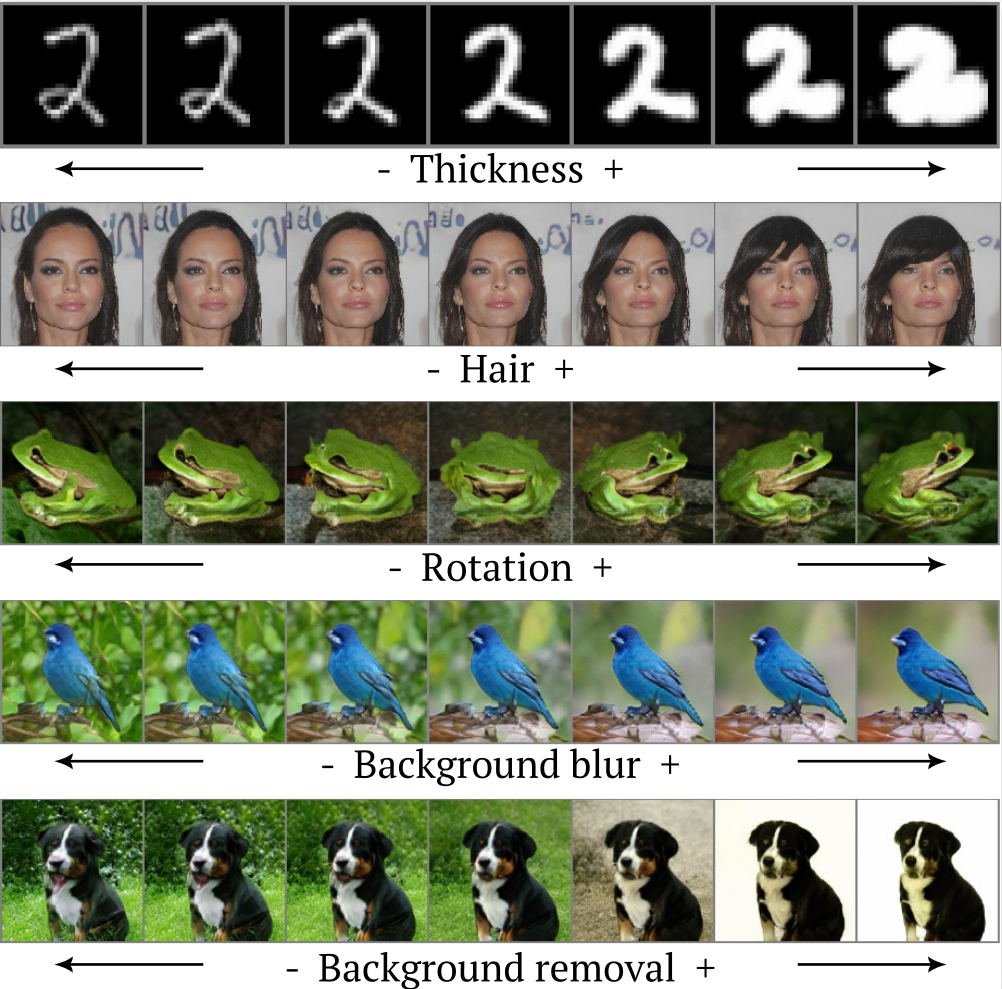
\includegraphics[width=1\textwidth]{pictures/tizer.png}}
        \end{minipage}
    \label{heat_maps}
    \end{figure}
    
\end{frame}

\end{document} 